\documentclass[a4paper,
12pt,
BCOR12mm,
]{scrartcl}
%scrreport
\usepackage[ngerman]{babel}
\usepackage[utf8]{inputenc}
\usepackage[T1]{fontenc}
\usepackage{url}
\usepackage[pdftex]{graphicx}
\usepackage{listingsutf8}
\usepackage{grffile}
\usepackage{epstopdf}
\usepackage{subfigure}

% lstlisting settings
\lstset{
showspaces=false,
breaklines=true,
breakindent=0pt,
frame=single,
language=C,
extendedchars=true,
inputencoding=utf8/latin1,
identifierstyle=\ttfamily,
basicstyle=\tiny,
numbers=left,
numberstyle=\tiny,
label=nodeadlock1
}

\title{APUVS, Blatt 3}
\author{Jan Fajerski and Kai Warncke and Magnus Müller}

\begin{document}
% NOTE: compile with pdflatex --shell-escape main.tex

\maketitle  
\section{Aufgabe 3.1}
\subsection{a)}
\begin{figure}[h!]
	\begin{center}
		\subfigure[fork (), Kindprozesse warten in Endlosschleife mit sleep ()]{
			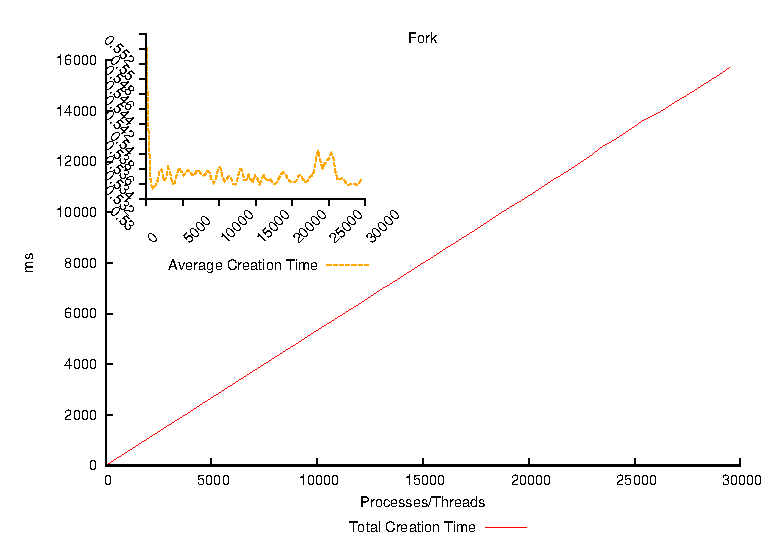
\includegraphics[scale=0.5]{../a_3_1/data/graphs/fork}
			\label{fig:fork_sleep}
		}
		\subfigure[fork () und exec ()]{
			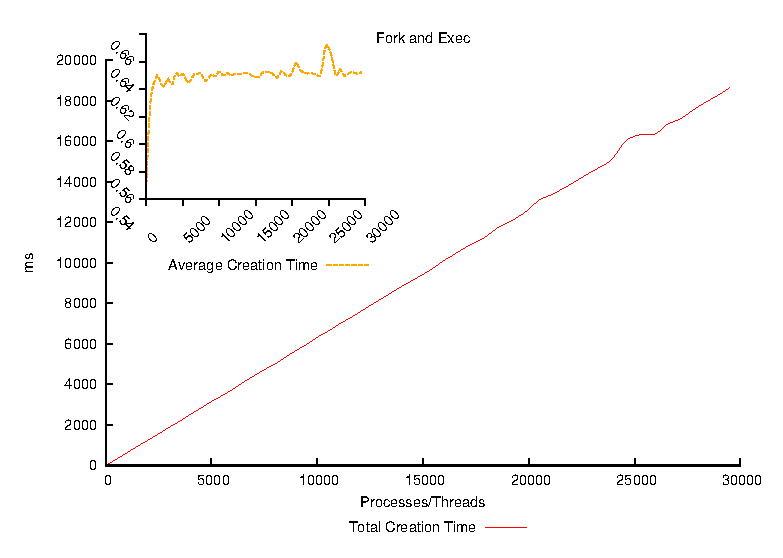
\includegraphics[scale=0.5]{../a_3_1/data/graphs/fork_exec}
			\label{fig:fork_exec}
		}
	\end{center}
\end{figure}

Wie an den Diagrammen \ref{fig:fork_sleep} und \ref{fig:fork_exec} zu erkennen ist,
benötigt die Erzeugung eines Prozesses per \verb|fork()| ca. $0.04ms$.
Hierbei ist zu beachten, dass \ref{fig:fork_exec} nur die Zeit zur Erstellung der Prozesse
misst, aber nicht die für \verb|exec()| benötigte Zeit. \\

% fork
% % awk '{sum=sum+$2;} END {printf sum/NR;}' fork.dat
% 3.16308e-05

\section{Aufgabe 3.2}
\subsection{b)}
\subsubsection{Prozesse}
vgl. angehängter Quelltext
	\begin{itemize}
		\item Starkes Thrasing
	\end{itemize}
\begin{figure}[h!]
	\begin{center}
		\subfigure[Kindprozesse arbeiten]{
			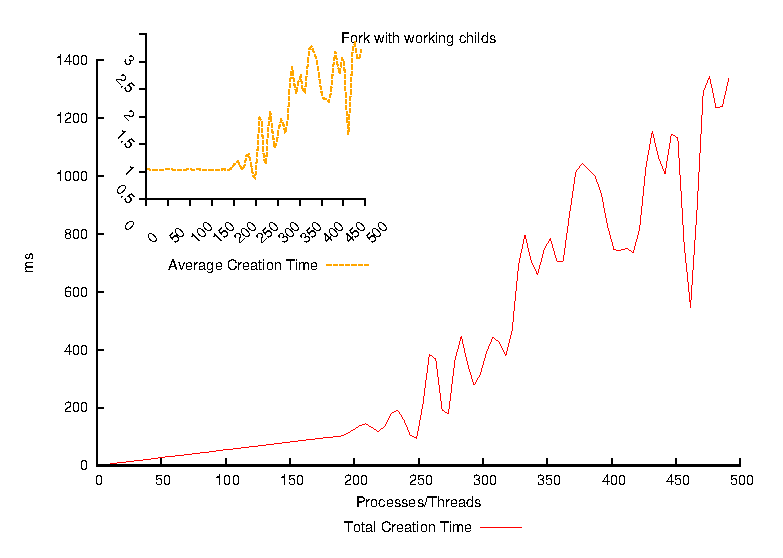
\includegraphics[scale=0.7]{../a_3_1/data/graphs/fork_childsworking}
			\label{fig:fork_childsworking}
		}
	\end{center}
\end{figure}

	\lstinputlisting[
	]
	{../a_3_1/fork/max_processes.c}
\end{document}
